\documentclass{article}
\usepackage[margin=1in]{geometry}
\usepackage{amsmath}
\usepackage{amssymb}
\usepackage{fancyhdr}
\usepackage{pgfplots}
\usepackage{graphicx}
\pgfplotsset{compat=1.16}

\author{Bryan Rodriguez-Andrade}
\title{Assignment 2 Part 1}

\pagestyle{fancy}
\renewcommand{\headrulewidth}{0pt}
\renewcommand{\footrulewidth}{0pt}

\fancyhf{}
\rhead{
    Bryan Rodriguez-Andrade\\
    CS 325 Fall 2020\\
    Homework 1\\
    \\
}
\rfoot{\thepage}

\begin{document}

\paragraph{1.}

$2/n, 37, \sqrt{n}, n, nloglogn, nlogn, nlog(n^2), nlog^2n, n^{1.5}, n^2, n^2logn, n^3, 2^{\frac{n}{2}}, 2^n$
 \\
 \\
$$nlog(n^2) = 2nlogn= O(nlogn)$$
$nlog(n^2)$ and nlogn grow at the same rate \\
 \\
\paragraph{2.} which grows faster? nlogn or $n^{1+\frac{\epsilon}{\sqrt{logn}}}$ when $\epsilon > 0$?\\
assume: f(x) $>$ g(x) and prove by contradition, where nlogn = f(x) and $n^{1+\frac{\epsilon}{\sqrt{logn}}}$ = g(x) \\

\begin{align*}
nlogn>n^{1+\frac{\epsilon}{\sqrt{logn}}}\\
n \cdot log n > n \cdot n^{\frac{\epsilon}{\sqrt{logn}}}\\
loglogn > logn^{\frac{\epsilon}{\sqrt{logn}}} = \frac{\epsilon}{\sqrt{logn}}logn\\
loglogn > \frac{\epsilon}{logn\frac{1}{2}} = \frac{\epsilon}{logn\frac{1}{2}} \cdot \frac{2logn}{2}\\
loglogn > \epsilon\sqrt{logn}\\
\text{let X = logn and we get} \\
\epsilon \sqrt{X}^ < logX\\
(\epsilon\sqrt{X})^2 < (logX)^2\\
\epsilon^2L < log^2L
\end{align*}
 \\
Because $\epsilon$ is a constant greater than 0, we can see from the above that $log^2X < \epsilon^2X$, this is then a contradiction to our statement above showing
that $n^{1+\frac{\epsilon}{\sqrt{logn}}}$ grows faster.\\

\paragraph{3.}\\
a. O(n)\\
b. O(n^2)\\
c. O(n^3)\\
d. O(n^2)\\
e. O(n^5)\\
f. O(n^4)


\begin{figure}
    \centering
    \caption{mergeTime table}
    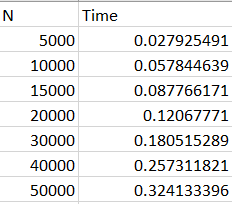
\includegraphics{CS325/Week_1/mergeTime.png}
    \caption{mergeTime graph}
    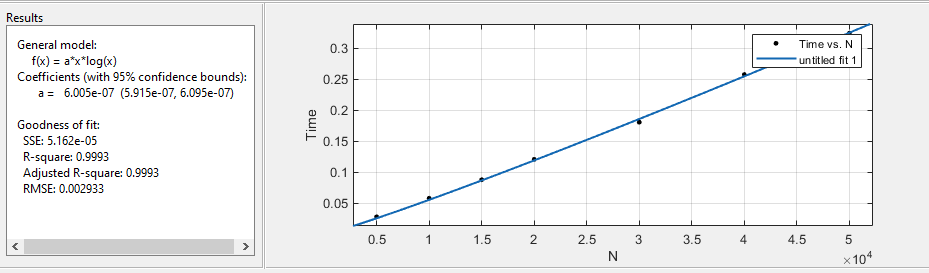
\includegraphics[width=\linewidth]{CS325/Week_1/mergeTimegraph.png}
\end{figure}

\begin{figure}
    \centering
    \caption{insertTime table}
    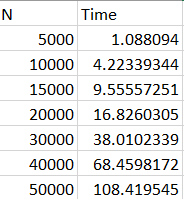
\includegraphics{CS325/Week_1/insertTime.png}
    \caption{insertTime graph}
    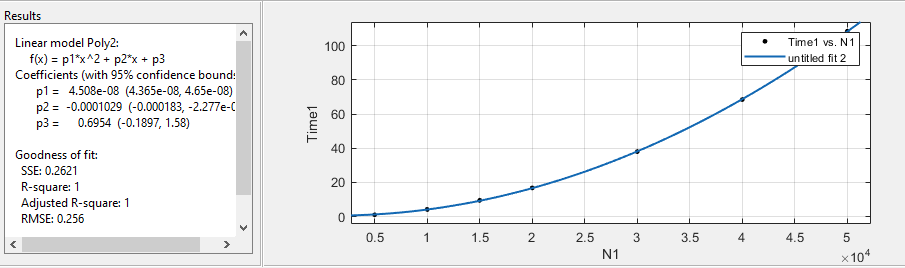
\includegraphics[width=\linewidth]{CS325/Week_1/insertTimegraph.png}
\end{figure}
\newpage

The merge sort equation that best fits the graph curve is an nlogn line, the best fit for the mergesort graph is an $n^2$ line.

\begin{figure}
    \centering
    \caption{combined algorithms graph}
    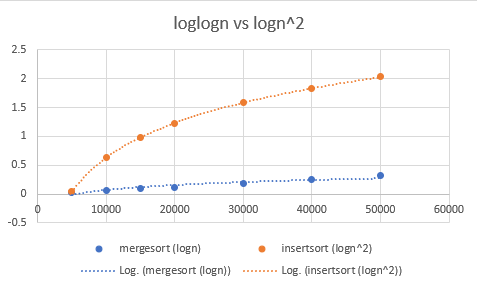
\includegraphics[width=\linewidth]{CS325/Week_1/combinedgraph.png}
\end{figure}
    
The experimental run times vs the theoretical running times of the algorithms compare closely of nlogn for Merge sort, and $n^2$ for insertion sort. The merge sort curve looks linear however, this is likely because the times are too close together to display a proper curve. This means that the variation of the run times was too small.  
\end{document}